\section{Eigenwerte und Eigenvektoren}

\subsection{Komplexe Zahlen}

Die Menge der komplexen Zahlen $\mathbb{C}$ erweitert die Menge der reellen Zahlen $\mathbb{R}$, so dass nun also auch Gleichungen der folgenden Art lösbar werden

$$
x^{2}+1=0
$$

Dafür wird die imaginäre Einheit $i$ mit der folgenden Eigenschaft eingeführt.

$$
i^{2}=-1
$$

Eine komplexe Zahl $z$ ist ein geordnetes Paar $(x, y)$ zweier Zahlen $x$ und $y$.

$$
z=x+i y
$$

Die imaginäre Einheit $i$ ist definiert durch

$$
i^{2}=-1
$$

Die Menge der komplexen Zahlen wird mit $\mathbb{C}$ bezeichnet

$$
\mathbb{C}=\{z \mid z=x+\text { iy mit } x, y \in \mathbb{R}\}
$$

Die reellen Bestandteile $x$ und $y$ von $z$ werden als Real- und Imaginärteil bezeichnet

\begin{itemize}
  \item Realteil von $z \quad \operatorname{Re}(z)=x$
  \item Imaginärteil von $z \quad \operatorname{Im}(z)=y$
\end{itemize}

Die zu $z$ konjugierte komplexe Zahl ist definiert als $z^{*}=x-i y$. Dies entspricht der an der $x$ - Achse gespiegelten Zahl.

Der Betrag einer komplexen Zahl ist definiert als $|z|=\sqrt{x^{2}+y^{2}}=\sqrt{z \cdot z^{*}}$. Dies entspricht der Länge des Zeigers.

\subsubsection*{Darstellungsformen}
\begin{itemize}
  \item Normalform $z=x+i y$
  \item Trigonometrische Form $z=r(\cos \varphi+i \cdot \sin \varphi)$
  \item Exponentialform $\quad z=r e^{i \varphi}$
\end{itemize}

$$
\begin{gathered}
x=r \cdot \cos \varphi, \quad y=r \cdot \sin \varphi, \quad r=\sqrt{x^{2}+y^{2}} \\
\varphi=\arcsin \left(\frac{y}{r}\right)=\arccos \left(\frac{x}{r}\right) \\
e^{i \varphi}=\cos \varphi+i \cdot \sin \varphi
\end{gathered}
$$

Beispiel

$$
z=3-11 i
$$

$$
\begin{gathered}
3=r \cdot \cos \varphi, \quad 11=r \cdot \sin \varphi, \quad r=\sqrt{3^{2}+11^{2}}=\sqrt{130} \\
\arcsin \left(\frac{11}{\sqrt{130}}\right)=\varphi=1.3
\end{gathered}
$$

$$
z=\cos (1.3)+i \cdot \sin (1.3), \quad z=\sqrt{130} \cdot e^{i \cdot 1.3}
$$

\begin{center}
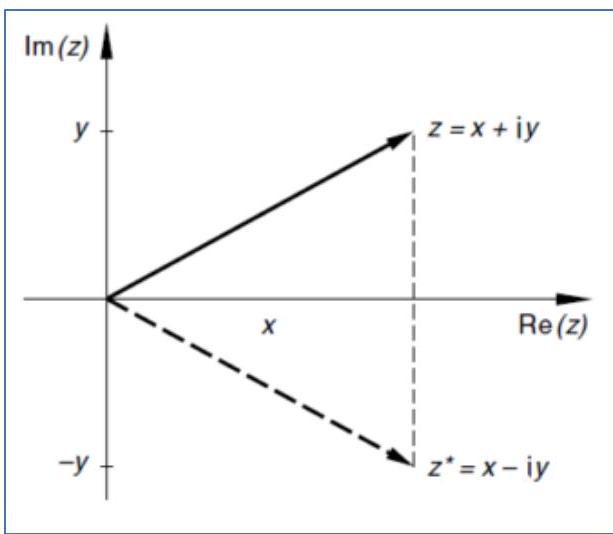
\includegraphics[width=\linewidth]{images/2024_12_29_68ccba06d0091c162fa4g-11}
\end{center}

\subsubsection*{Grundrechenarten}
Es sei $z_{1}=x_{1}+i y_{1}$ und $z_{2}=x_{2}+i y_{2}$

\begin{itemize}
  \item Summation $z_{1}+z_{2}=\left(x_{1}+x_{2}\right)+i\left(y_{1}+y_{2}\right)$
  \item Subtraktion $z_{1}-z_{2}=\left(x_{1}-x_{2}\right)+i\left(y_{1}-y_{2}\right)$
\end{itemize}

Multiplikation

$$
\begin{gathered}
z_{1} \cdot z_{2}=\left(x_{1} x_{2}-y_{1} y_{2}\right)+i\left(x_{1} y_{2}+x_{2} y_{1}\right) \\
z_{1} \cdot z_{2}=r_{1} e^{i \varphi_{1}} \cdot r_{2} e^{i \varphi_{2}}=r_{1} r_{2} e^{i\left(\varphi_{1}+\varphi_{2}\right)}
\end{gathered}
$$

Division

$$
\begin{gathered}
\frac{z_{1}}{z_{2}}=\frac{z_{1} \cdot z_{2}^{*}}{z_{2} \cdot z_{2}^{*}}=\frac{\left(x_{1}+i y_{1}\right)\left(x_{2}-i y_{2}\right)}{\left(x_{2}+i y_{2}\right)\left(x_{2}-i y_{2}\right)} \\
=\frac{\left(x_{1} x_{2}+y_{1} y_{2}\right)+i\left(y_{1} x_{2}-x_{1} y_{2}\right)}{x_{2}^{2}+y_{2}^{2}}=\frac{\left(x_{1} x_{2}+y_{1} y_{2}\right)}{x_{2}^{2}+y_{2}^{2}}+i \frac{\left(y_{1} x_{2}-x_{1} y_{2}\right)}{x_{2}^{2}+y_{2}^{2}}
\end{gathered}
$$

$$
\frac{z_{1}}{z_{2}}=\frac{r_{1} e^{i \varphi_{1}}}{r_{2} e^{i \varphi_{2}}}=\frac{r_{1}}{r_{2}} e^{i\left(\varphi_{1}+\varphi_{2}\right)}
$$

\subsubsection*{Potenzieren und Radizieren}
Die $n$-te Potenz einer komplexen Zahl lässt sich einfach berechnen, wenn diese in der trigonometrischen oder der Exponentialform vorliegt (Sei $n \in \mathbb{N}$ ):

$$
z=r \cdot e^{i \varphi} \rightarrow z^{n}=\left(r e^{i \varphi}\right)^{n}=r^{n} e^{i n \varphi}=r^{n}(\cos (n \varphi)+i \cdot \sin (n \varphi))
$$

Fundamentalgesetz der Algebra\\
Eine algebraische Gleichung $n$-ten Grades mit komplexen Koeffizienten und Variablen $a_{i}, z \in \mathbb{C}$

$$
a_{n} z^{n}+a_{n-1} z^{n-1}+\cdots+a_{1} z+a_{0}=0
$$

Besitzt in der Menge $\mathbb{C}$ der komplexen Zahlen genau $n$ Lösungen

\subsubsection*{Wurzel einer komplexen Zahl}
Eine komplexe Zahl $z$ wird als $n$-te Wurzel von $a \in \mathbb{C}$ bezeichnet, wenn

$$
z^{n}=a \rightarrow z=\sqrt[n]{a}
$$

Lösungen der algebraischen Gleichung $z^{n}=a$

$$
z^{n}=a=r_{0} e^{i \varphi}\left(r_{0}>0 ; n=2,3,4, \ldots\right)
$$

Besitzt in der Menge $\mathbb{C}$ genau $n$ verschiedene Lösungen (Wurzeln)

$$
\begin{gathered}
z_{k}=r\left(\cos \varphi_{k}+i \cdot \sin \varphi_{k}\right)=r e^{i \varphi_{k}} \\
r=\sqrt[n]{r_{0}}, \quad \varphi_{k}=\frac{\varphi+k \cdot 2 \pi}{n}, \quad(f \ddot{u} r k=0,1,2, \ldots, n-1)
\end{gathered}
$$

Die zugehörigen Bildpunkte liegen in der komplexen Zahlenebene auf einem Kreis um den Nullpunkt mit dem Radius $r=\sqrt[n]{r_{0}}$ und bilden die Ecken eines regelmässigen $n$-Ecks.


\subsection{Intro EW und EV}

Es sei $A \in \mathbb{R}^{n \times n} . \lambda \in \mathbb{C}$ heisst Eigenwert von $A$, wenn es einen Vektor $x \in \mathbb{C}^{n} \backslash\{0\}$ gibt mit

$$
A x=\lambda x
$$

$x$ heisst dann Eigenvektor von $A$.

\subsubsection*{Eigenschaften von Eigenwerten}
$$
A x-\lambda x=0 \Leftrightarrow\left(A-\lambda I_{n}\right) \cdot x=0
$$

Die Eigenwerte einer Diagonal- oder eine Dreiecksmatrix sind deren Diagonalelemente.

\subsubsection*{Polynom und Spur}
Es sei $A \in \mathbb{R}^{n \times n}, \lambda \in \mathbb{C}$. Dann gilt

$$
\lambda \text { ist ein Eigenwert von } A \Leftrightarrow \operatorname{det}\left(A-\lambda I_{n}\right)=0
$$

Die Abbildung $p$ ist definiert durch

$$
p(\lambda) \rightarrow \operatorname{det}\left(A-\lambda I_{n}\right)
$$

Ist ein Polynom vom Grad $n$ und wird charakteristisches Polynom von $A$ genannt. Die Eigenwerte von $A$ sind also die Nullstellen des charakteristischen Polynoms. Damit hat $A$ also genau $n$ Eigenwerte, von denen manche mehrfach vorliegen können.

Die Determinante der Matrix $A$ ist gerade das Produkt ihrer Eigenwerte $\lambda_{1}, \ldots, \lambda_{n}$. Die Summe der Eigenwerte ist gleich der Summe der Diagonalelemente von $A$, d.h. gleich der Spur (tr) von $A$ :

\begin{itemize}
  \item $\operatorname{det}(A)=\lambda_{1} \cdot \lambda_{2} \cdot \ldots \cdot \lambda_{n}$
  \item $\operatorname{tr}(A)=a_{11}+a_{22}+\cdots+a_{n n}=\lambda_{1}+\lambda_{2}+\cdots+\lambda_{n}$
\end{itemize}

Ist $\lambda_{i}$ ein Eigenwert der regulären Matrix $A$, so ist der Kehrwert $\frac{1}{\lambda_{i}}$ ein Eigenwert der inversen Matrix $A^{-1}$.

\subsubsection*{Vielfachheit und Spektrum}
Es sei $A \in \mathbb{R}^{n \times n}$. Die Vielfachheit, mit der $\lambda$ als Nullstelle des charakteristischen Polynoms von $A$ auftritt, heisst algebraische Vielfachheit von $\lambda$.

Das Spektrum $\sigma(A)$ ist die Menge aller Eigenwerte von $A$.

\subsubsection*{Beispiel}
Berechne Spektrum, Determinante und Spur von

$$
A=\left(\begin{array}{lll}
1 & 0 & 0 \\
2 & 3 & 0 \\
0 & 1 & 2
\end{array}\right)
$$

Eigenwerte

$$
\lambda_{1}=1, \quad \lambda_{2}=3, \quad \lambda_{3}=2
$$

Determinante

$$
\operatorname{det}(A)=\lambda_{1} \cdot \lambda_{2} \cdot \lambda_{3}=6
$$

Spur

$$
\operatorname{tr}(A)=\lambda_{1}+\lambda_{2}+\lambda_{3}=6
$$

Spektrum

$$
\sigma(A)=3
$$

\subsubsection*{Eigenschaften von Eigenvektoren}
Seien zwei Eigenvektoren $x, y$ zum selben Eigenwert $\lambda \in \mathbb{C}$ einer Matrix $A \in \mathbb{R}^{n} \times \mathbb{R}^{n}$, so ist $x+y$ und auch jedes Vielfach von $x$ ebenfalls ein Eigenvektor zum Eigenwert $\lambda$ :

$$
\begin{gathered}
A(x+y)=A x+A y=\lambda x+\lambda=\lambda(x+y) \\
A(\mu x)=\mu A x=\mu \lambda x=\lambda \mu x
\end{gathered}
$$

\subsubsection*{Eigenraum}
Sei $\lambda \in \mathbb{C}$ ein Eigenwert von $A \in \mathbb{R}^{n \times n}$. Dann bilden die Eigenvektoren zum Eigenwert $\lambda$ zusammen mit dem Nullvektor 0 einen Unterraum von $\mathbb{C}^{n}$, den sogenannten Eigenraum

Der Eigenraum des Eigenwertes $\lambda$ ist die Lösungsmenge des homogenen LGS

$$
\left(A-\lambda I_{n}\right) x=0
$$

Welches nur dann eine nicht-triviale Lösung aufweist, wenn $r g\left(A-\lambda I_{n}\right)<n$.\\
Die Dimension des Eigenraumes von $\lambda$ wird die geometrische Vielfachheit von $\lambda$ genannt. Sie berechnet sich als

$$
n-r g\left(A-\lambda I_{n}\right)
$$

Und gibt die Anzahl der lin. Unabhängigen Eigenvektoren zum Eigenwert $\lambda$.\\
Geometrische und algebraische Vielfachheit eines Eigenwerts müssen nicht gleich sein. Die geom. Vielfachheit ist aber stets kleiner oder gleich der algebraischen Vielfachheit.

Beispiel: Berechne Eigenwerte, Eigenvektoren, Eigenräume

$$
\begin{gathered}
A=\left(\begin{array}{cc}
2 & 5 \\
-1 & -2
\end{array}\right), \quad A-\lambda I_{n}=\left(\begin{array}{cc}
2-\lambda & 5 \\
-1 & -2-\lambda
\end{array}\right) \\
p(\lambda)=\operatorname{det}\left(A-\lambda I_{n}\right)=(2-\lambda)(-2-\lambda)-5 \cdot-1 \\
p(\lambda)=-4+\lambda^{2}+5=\lambda^{2}+1=0 \\
\lambda^{2}=-1=i^{2}
\end{gathered}
$$

Eigenwerte

$$
\lambda_{1}=i, \quad \lambda_{2}=-i
$$

Eigenvektor für $\boldsymbol{\lambda}_{\mathbf{1}}=\boldsymbol{i}$

$$
\begin{gathered}
\left(\begin{array}{cc}
2-i & 5 \\
-1 & -2-i
\end{array}\right) \rightarrow\left(\begin{array}{cc}
2-i & 5 \\
0 & -2-i+\frac{5}{2-i}
\end{array}\right) \\
-2-i+\frac{5}{2-i}=(2-i)(-2-i)+5=1+i^{2}=0 \\
0=(2-i) \cdot x_{1}+5 \cdot x_{2} \\
x_{1}=-\frac{5 x_{2}}{2-i} \cdot \frac{2+i}{2+i}=-\frac{5 \cdot(2+i)}{4-i^{2}}=-\frac{10+5 i}{5}=-2-i \\
x_{1}=\binom{-2-i}{1}
\end{gathered}
$$

Eigenraum

$$
\begin{gathered}
E_{\lambda_{1}}=\left\{x \left\lvert\, x=\mu=\binom{-2-i}{1}\right., \mu \in \mathbb{R}\right\} \\
E_{\lambda_{2}}=\left\{x \left\lvert\, x=\mu=\binom{-2+i}{1}\right., \mu \in \mathbb{R}\right\}
\end{gathered}
$$

\subsection{Numerische Berechnung EW und EV}

\subsubsection*{Ähnliche Matrizen / Diagonalisierbarkeit}
Es seien $A, B \in \mathbb{R}^{n \times n}$ und $T$ eine reguläre Matrix mit ... so heissen $B$ und $A$ zueinander ähnliche Matrizen.

$$
B=T^{-1} A T
$$

Im Spezialfall, dass $B=D$ ein Diagonalmatrix ist, also ... nennt man $A$ diagonalisierbar.

$$
D=T^{-1} A T
$$

\subsubsection*{Eigenwerte und Eigenvektoren ähnlicher / diagonalisierbarer Matrizen}
Es seien $A, B \in \mathbb{R}^{n \times n}$ zueinander ähnliche Matrizen. Dann gilt

\begin{enumerate}
  \item $A$ und $B$ haben dieselben Eigenwerte, inkl. deren algebraische Vielfachheit
  \item Ist $x$ ein Eigenvektor zum Eigenwert $\lambda$ von $B$, dann ist $T x$ ein Eigenvektor zum Eigenwert $\lambda$ von $A$.
  \item Falls $A$ diagonalisierbar ist
\end{enumerate}

\begin{itemize}
  \item Diagonalelemente von $D$ sind die Eigenwerte von $A$
  \item Die linear unabhängigen Eigenvektoren von $A$ stehen in den Spalten von $T$
\end{itemize}

Der Spektralradius $p(A)$ einer Matrix $A \in \mathbb{R}^{n \times n}$ ist definiert als

$$
p(A)=\max \left\{|\lambda| \mid \lambda \text { ist ein Eigenwert von } A \in \mathbb{R}^{n \times n}\right\}
$$

Sei $A \in \mathbb{R}^{n \times n}$ eine diagonalisierbare Matrix mit den Eigenwerten $\lambda_{1}, \ldots, \lambda_{n}$ und dem betragsmässig grössten Eigenwert $\lambda_{1}$ mit

$$
\left|\lambda_{1}\right|>\left|\lambda_{2}\right| \geq \cdots \geq\left|\lambda_{n}\right|
$$

\subsubsection*{Vektoriteration / von-Mises-Iteration}
So konvergieren für (fast) jeden Startvektor $v^{(0)} \in \mathbb{C}^{n}$ mit Länge 1 die Folgen

$$
v^{(k+1)}=\frac{A v^{(k)}}{\left\|A v^{(k)}\right\|_{2}}, \quad \lambda^{(k+1)}=\frac{\left(v^{(k)}\right)^{T} A v^{(k)}}{\left(v^{(k)}\right)^{T} v^{(k)}}
$$

Für $k \rightarrow \infty$ gegen einen Eigenvektor $v$ zum Eigenwert $\lambda_{1}$ von $A$ (also $v^{(k)} \rightarrow v$ und $\lambda^{(k)} \rightarrow \lambda_{1}$ )

\subsubsection*{$Q R$-Verfahren}
Sei $A \in R^{n \times n}$

$$
A_{0}:=A, \quad P_{0}:=I_{n}
$$

Für $i=0,1,2, \ldots$

\begin{itemize}
  \item $A_{i}:=Q_{i} \cdot R_{i}$\\
$Q R$-Zerlegung von $A_{i}$
  \item $A_{i+1}:=R_{i} \cdot Q_{i}$
  \item $P_{i+1}:=P_{i} \cdot Q_{i}$
\end{itemize}

